\chapter{Literature Review}
\vspace{-1cm}
This chapter presents a literature review that examines the current body of knowledge surrounding Automated Machine Learning (AutoML), ML lifecycle management, and no-code AI platforms. The review synthesizes findings from key academic papers published in Springer and IEEE to explore the core principles, implementation strategies, and challenges within end-to-end machine learning automation. It specifically focuses on foundational concepts like automated model selection, data preprocessing pipelines, ML operations (MLOps), and the evolution towards fully automated, user-accessible ML systems. This analysis provides a foundational context for the InferX ML project by highlighting established practices, identifying existing gaps, and justifying the need for a no-code, explainable AutoML platform.



\section{Comparative Analysis of Literature Review}

Automated Machine Learning (AutoML) has gained significant attention as a means to reduce the manual effort involved in designing, training, and evaluating machine learning models. A survey by Springer (2024), titled ``Automated Machine Learning: Past, Present and Future,'' outlines the evolution of AutoML from hyperparameter optimization to end-to-end automation. It categorizes AutoML into tasks such as data preprocessing, feature engineering, algorithm selection, and neural architecture search. Despite advancements, the study highlights the lack of unified, user-friendly platforms for non-technical users. This gap motivates InferX ML, which integrates these components into a single no-code platform with rule-based automation and AI-driven goal analysis. [1]\vspace{0.3cm}

The operational aspect of ML systems is explored in Springer (2025) in ``Machine Learning Operations Landscape: Platforms and Tools.'' The paper reviews MLOps platforms supporting lifecycle automation, including training, versioning, and deployment. While tools like Vertex AI, SageMaker, and MLflow provide strong capabilities, they are complex and resource-intensive. The study emphasizes the need for lightweight and accessible alternatives. InferX ML addresses this by offering a containerized, open-source architecture using Flask, Celery, MinIO, and PostgreSQL. [2]\vspace{0.3cm}

Springer (2025) in ``Resilient Automatic Model Selection for Mobility Prediction'' demonstrates that automated and rule-based model selection can match or outperform manually tuned models, especially with dynamic data. This supports InferX ML’s approach of automatically selecting suitable algorithms such as Random Forest, XGBoost, ARIMA, Prophet, LSTM, MobileNet, and EfficientNet based on dataset characteristics and problem type. [3]\vspace{0.3cm}

The IEEE paper ``Automated Retraining of Machine Learning Models'' (2019) highlights the importance of maintaining model performance through automated retraining as new data becomes available. While InferX ML currently focuses on initial model training, its architecture using Celery and MinIO provides a strong foundation for future retraining capabilities. [4]\vspace{0.3cm}

The concept of full lifecycle management is discussed in the IEEE paper ``ModelOps: Cloud-Based Lifecycle Management for AI'' (2019), which extends DevOps principles to ML systems. It promotes microservices-based architectures for managing model lifecycles. InferX ML aligns with this approach through its modular design using Flask, Celery, Redis, MinIO, PostgreSQL, React, and Streamlit, orchestrated via Docker Compose. [5]
\begin{figure}[H]
    \centering
    \fbox{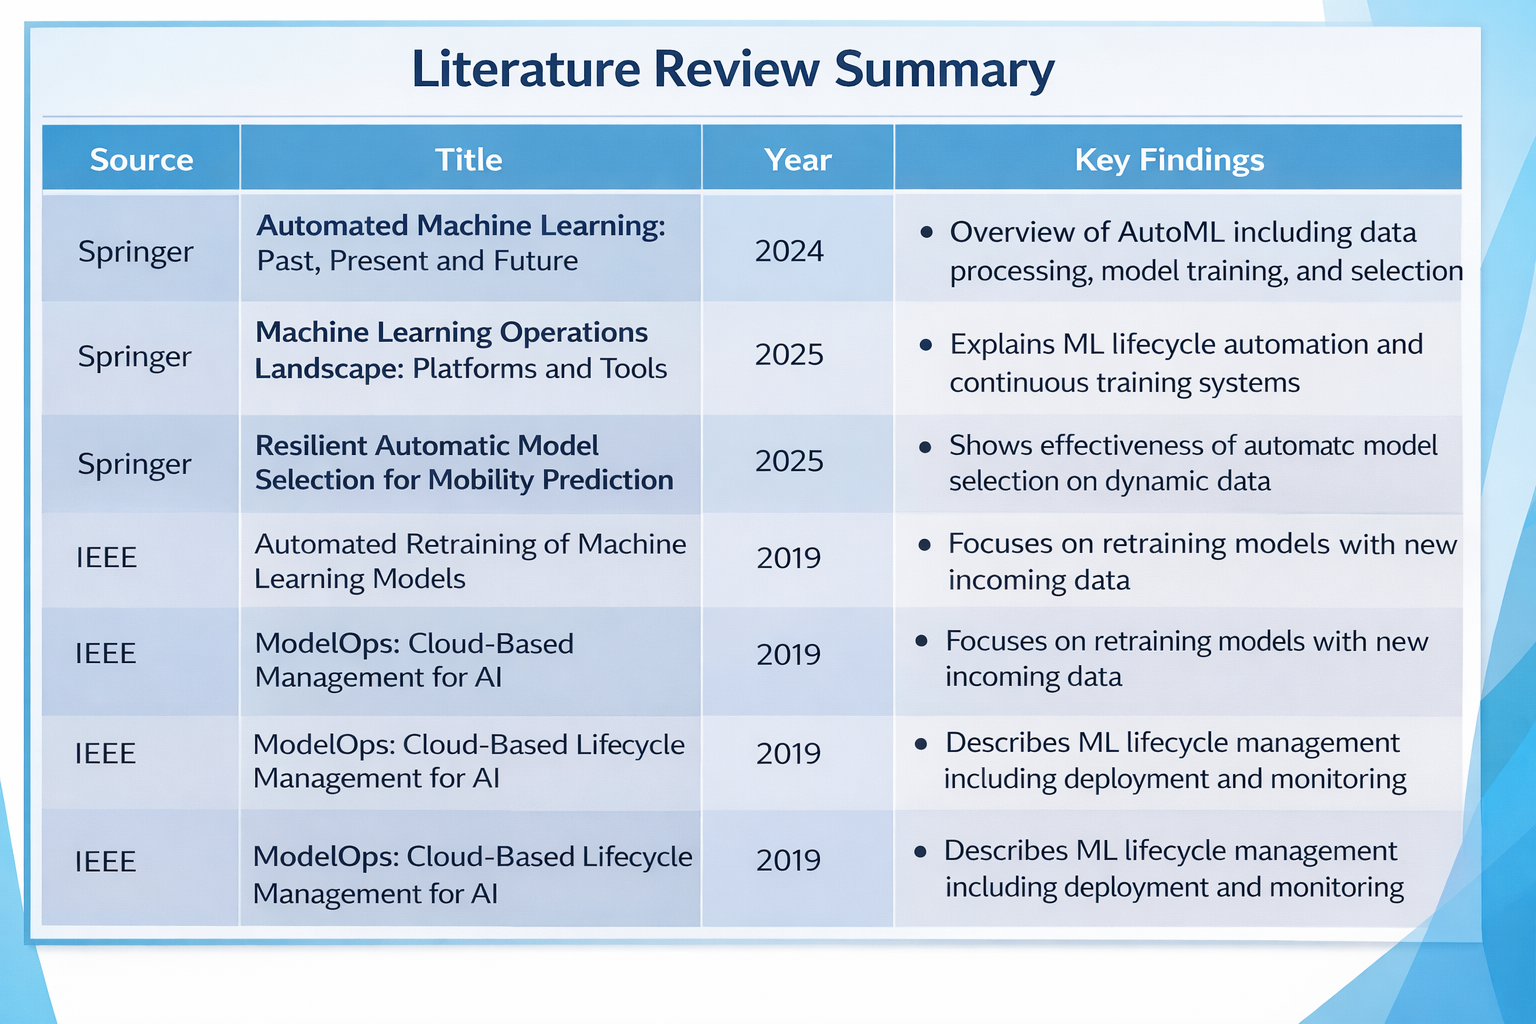
\includegraphics[width=1\textwidth]{images/1.png}}
    \caption{Comparative Analysis of Literature Review}
    \label{fig:img5}
\end{figure}

